\section{Results}
\label{sec:results}

\begin{figure}[t]
\centering
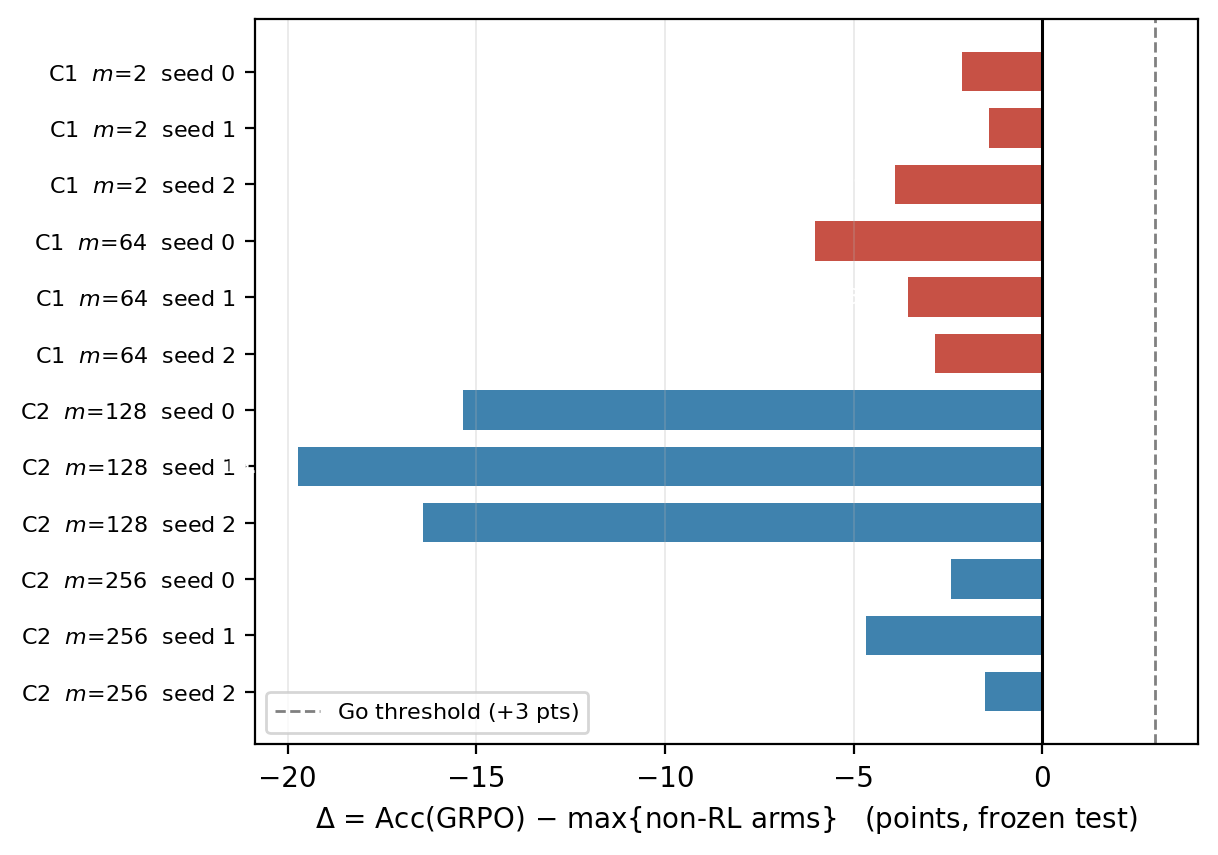
\includegraphics[width=\columnwidth]{figs/F2_delta.png}
\caption{Frozen-test $\Delta$ for all 17 groups, grouped by backbone. Every
value is negative and none approaches the pre-registered $+3$-point Go
threshold (dashed). The arm attaining $\max \mathcal{B}$ is annotated per
band: the solver at 0.5B and 1B, continued SFT at 7B.}
\label{fig:delta}
\end{figure}

\begin{table}[t]
\centering
\small
\setlength{\tabcolsep}{3.2pt}
\caption{Frozen-test accuracy (\%) per arm and $\Delta$ (points) at 0.5B and
1B. The maximum over $\mathcal{B}$ is attained by the solver in all 11 groups.
Config~2 $m{=}128$ seed~1 is excluded: its GRPO run ended with zero positive
reward (Section~\ref{sec:analysis}).}
\label{tab:main}
\begin{tabular}{rr rrrrr r}
\toprule
$m$ & seed & solver & $W_m$ & c-SFT & RS-SFT & GRPO & $\Delta$ \\
\midrule
\multicolumn{8}{l}{\textit{Config~1: CodeTAT-QA $\times$ Qwen2.5-0.5B ($n{=}282$)}} \\
2  & 0 & \textbf{64.54} & 15.60 & 24.47 & 27.66 & 62.41 & $-2.13$ \\
2  & 1 & \textbf{64.54} & 14.54 & 18.09 & 28.01 & 63.12 & $-1.42$ \\
2  & 2 & \textbf{64.54} & 26.60 & 20.57 & 30.50 & 60.64 & $-3.90$ \\
64 & 0 & \textbf{64.54} & 29.43 & 43.62 & 51.06 & 58.51 & $-6.03$ \\
64 & 1 & \textbf{64.54} & 27.66 & 45.39 & 56.03 & 60.99 & $-3.55$ \\
64 & 2 & \textbf{64.54} & 32.62 & 45.74 & 51.42 & 61.70 & $-2.84$ \\
\midrule
\multicolumn{8}{l}{\textit{Config~2: CodeFinQA $\times$ Llama-3.2-1B ($n{=}664$)}} \\
128 & 0 & \textbf{32.38} & 12.05 & 20.18 & 21.84 & 17.02 & $-15.36$ \\
128 & 2 & \textbf{32.53} & 12.65 & 18.83 & 25.00 & 16.11 & $-16.42$ \\
256 & 0 & \textbf{32.38} & 25.60 & 26.36 & 28.92 & 29.97 & $-2.41$ \\
256 & 1 & \textbf{32.83} & 25.75 & 27.11 & 25.90 & 28.16 & $-4.67$ \\
256 & 2 & \textbf{32.08} & 28.16 & 27.41 & 30.27 & 30.57 & $-1.51$ \\
\bottomrule
\end{tabular}
\end{table}

\subsection{Every frozen-test effect size is negative}

Table~\ref{tab:main} and Figure~\ref{fig:delta} give the small-backbone result:
11 groups, $\Delta$ from $-1.42$ to $-16.42$ points, mean $-5.48$. No group
approaches the pre-registered $+3$-point threshold. Adding the six 7B groups of
Section~\ref{sec:scale} gives 17 negative values out of 17, mean $-4.44$.

The two configurations differ in dataset family, model family, and absolute
difficulty---the solver scores $64.54\%$ on Config~1 and $32.08$--$32.83\%$ on
Config~2---yet agree in sign. Config~2 at $m{=}128$ is significant under
McNemar after Holm correction ($p < 0.001$).

One group deserves note for a reason unrelated to $\Delta$: at Config~2
$m{=}128$, GRPO ($16.11$--$17.02\%$) falls below continued SFT
($18.83$--$20.18\%$) and RS-SFT ($21.84$--$25.00\%$). Here the verdict is
negative even without the solver---the learning-only control group already
suffices.

\subsection{Why: the scarce regime is the non-learner's regime}

\begin{figure}[t]
\centering
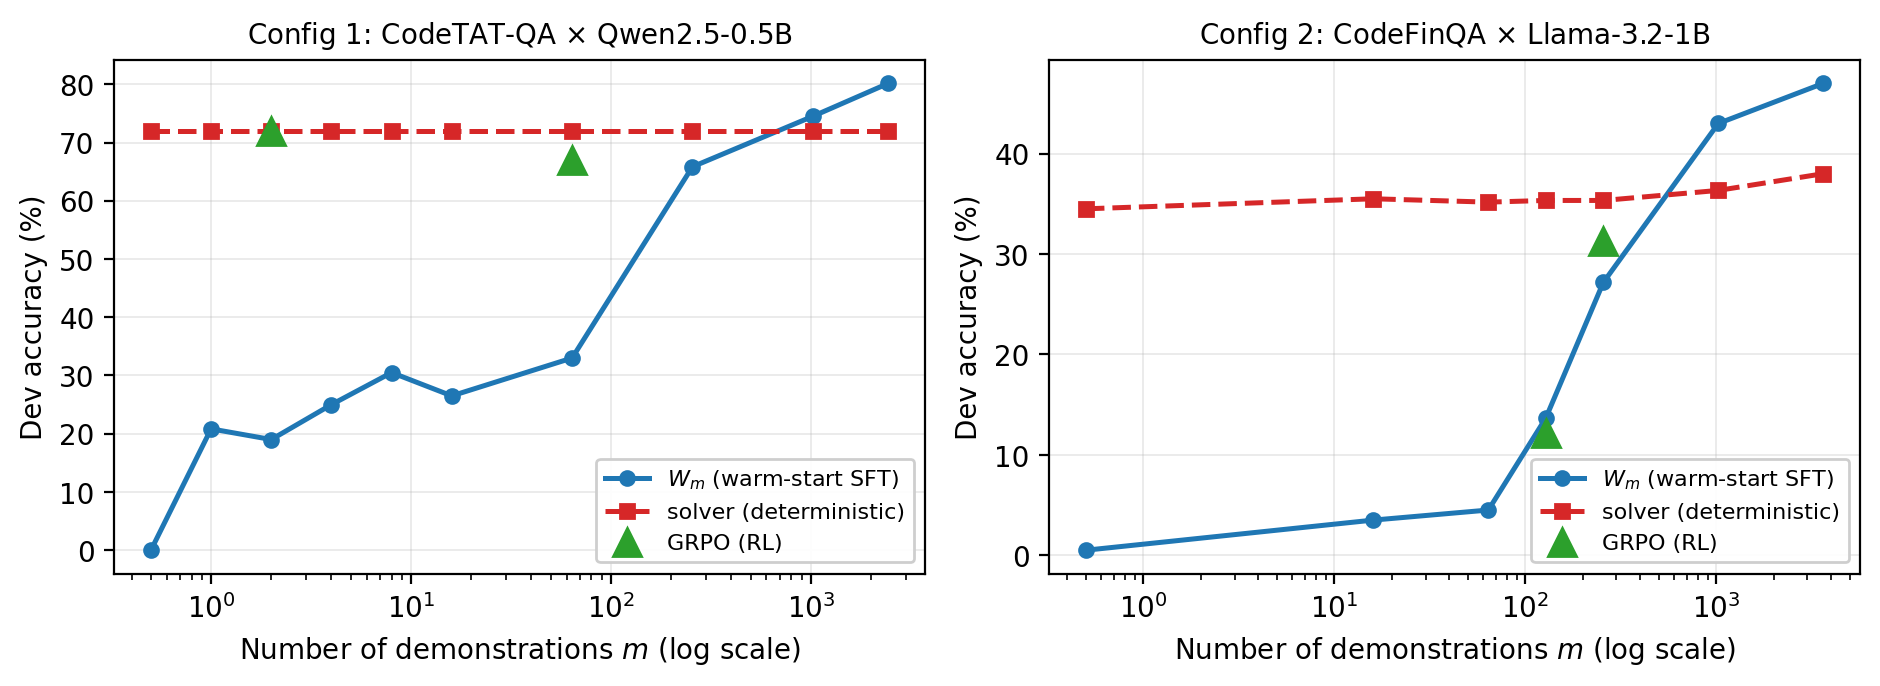
\includegraphics[width=\columnwidth]{figs/F1_dose_curve.png}
\caption{Dose--response curves (dev; three seeds at the operating budgets, one
seed at the diagnostic-only budgets). Learning arms scale with the
demonstration budget; the deterministic solver does not.}
\label{fig:dose}
\end{figure}

Figure~\ref{fig:dose} explains the sign at small scale. Warm-start accuracy in
Config~1 climbs from $0.0\%$ at $m{=}0$ through $19.0\%$ ($m{=}2$), $33.0\%$
($m{=}64$) and $65.8\%$ ($m{=}256$) to $80.2\%$ at the full pool; Config~2
climbs from $0.5\%$ to $47.0\%$. The solver consumes no parameters and learns
nothing: it scores $72.0\%$ at \emph{every one} of Config~1's ten budgets, and
stays within $34.5$--$38.0\%$ across Config~2's seven.

The crossing points matter. In Config~1 the learning curve does not overtake
the solver until $m{=}1024$ ($74.5\%$ vs.\ $72.0\%$); at $m{=}256$ it is still
behind at $65.8\%$. Config~2 crosses near $m{=}1024$ as well ($43.0\%$ vs.\
$36.3\%$). Everything left of that crossing is the demonstration-scarce
regime---the regime in which RLVR is most often argued to be valuable, and in
which a method that ignores demonstrations entirely is hardest to beat.

\subsection{The gain is real; the conclusion is not}

Against a warm-start-only control the same runs look excellent: on dev, GRPO
improves over $W_m$ from $19.0\%$ to $72.0\%$ at $m{=}2$ and from $33.0\%$ to
$67.0\%$ at $m{=}64$. Both would be reported as large positive results. Adding
one non-learning arm to the same comparison turns every frozen-test verdict
negative. RL is doing real work here---it beats every learning baseline by up
to 35 points---but ``does RL beat SFT?'' and ``is RL the best use of this
demonstration budget?'' have different answers.

\subsection{Dev selection bias, observed three times}

On dev, two groups produced non-negative values: Config~1 $m{=}2$ gave
$\Delta = +0.00$, $-0.50$, $+0.50$. The same three groups on the frozen test
gave $-2.13$, $-1.42$, $-3.90$. Two further instances appear later: the
$\beta{=}0$ hyperparameter setting (Section~\ref{sec:analysis}) yields
$+1.50$ on dev and $-2.13$ on test, and the 7B $m{=}2$ seed-2 group yields
$+1.50$ on dev and $-1.77$ on test. In all three, dev favors GRPO and the
frozen test does not.

Since every checkpoint in every arm is selected on dev, the arm whose dev
trajectory fluctuates most gains the most from that selection---and a
policy-gradient run plausibly fluctuates more than a fine-tuning run. We state
this as a candidate mechanism rather than a measured one: three instances
identified after the fact do not establish it, and our stored artifacts support
the per-arm dev-checkpoint variance it predicts only at 7B
(Section~\ref{sec:discussion}). What the three instances do show without
interpretation is the practical point: without a frozen test set we would have
reported non-negative results in three groups and a positive one from the
sweep. All $17 \times 5 = 85$ arm evaluations of the reported groups are
present; nothing in $\mathcal{B}$ is imputed or dropped.

